\chapter{排版示例:『大学物理学1』期中试题解答}
\date{闭卷,允许携带\underline{\textbf{无存储功能的计算器}}入场}{\zhtoday}{299792458}{大学物理教学团队}
\section{选择题(每题3分,共30分)}
{
\begin{choice}{D}{加速度}
    某质点作直线运动的运动学方程为$x=6t-2t^3+6\ (\mathrm{SI})$,则该质点作
    \begin{tasks}(2)
        \task 匀加速直线运动,加速度沿$x$轴正方向
        \task 匀加速直线运动,加速度沿$x$轴负方向
        \task 变加速直线运动,加速度沿$x$轴正方向
        \task 变加速直线运动,加速度沿$x$轴负方向
    \end{tasks}
\end{choice}
\begin{solution}
    质点的加速度$a=\frac{\d^2 x}{\d t^2}=-12t\ (\mathrm{SI})<0$.\sokka{D}
\end{solution}

\hspace{-2.16em}
\begin{minipage}{0.67\textwidth}
\begin{choice}{D}{功}
    如图所示,木块$m$沿固定的光滑斜面下滑,当下降$h$高度时,重力做功的瞬时功率是
    \begin{tasks}(2)
        \task $mg\sqrt{2gh}$
        \task $mg\cos{\theta}\sqrt{2gh}$
        \task $mg\sin{\theta}\sqrt{\frac{1}{2}gh}$
        \task $mg\sin{\theta}\sqrt{2gh}$
    \end{tasks}
\end{choice}
\end{minipage}
\hfill
\begin{minipage}[c]{0.33\textwidth}
\begin{center}
    \begin{tikzpicture}
    \draw [thick] (4,0)--(0,0)--(3.2,2.4);
    \coordinate (a) at (4,0);
    \coordinate (o) at (0,0);
    \coordinate (b) at (3.2,2.4);
    \pic["$\theta$", draw=red!80!green!60!, ultra thick, angle
eccentricity=1.35, angle radius=24]{angle=a--o--b};
    \draw [rotate=36.8,thick,densely dashed] (0.5,0)--(1.3,0)--(1.3,0.5)--(0.5,0.5)--cycle;
    \draw [rotate=36.8,thick] (2.3,0)--(3.1,0)--(3.1,0.5)--(2.3,0.5)--cycle;
    \end{tikzpicture}
\end{center}
\end{minipage}
\begin{solution}
    下落高度$h$时,木块的速度大小$v=\sqrt{2gh}$.此时重力的功率
    $$P=\boldsymbol{F}\cdot\boldsymbol{v}=mg\sin{\theta}\sqrt{2gh}$$
    \sokka{D}
\end{solution}

\hspace{-2.16em}
\begin{minipage}{0.67\textwidth}
\begin{choice}{B}{保守力}
    一物体挂在一弹簧下面,平衡位置在$O$点,现用手向下拉物体,第一次把物体由$O$点拉到$M$点,第二次由$O$点拉到$N$点,再由$N$点送回$M$点.则在这两个过程中
    \begin{tasks}
        \task 弹性力做功相等,重力做功不相等
        \task 弹性力做功相等,重力做功也相等
        \task 弹性力做功不相等,重力做功相等
        \task 弹性力做功不相等,重力做功也不相等
    \end{tasks}
\end{choice}
\end{minipage}
\hfill
\begin{minipage}[c]{0.33\textwidth}
\begin{center}
    \begin{tikzpicture}
        \filldraw [pattern=north west lines] (-1,0)--(1,0)--(1,0.2)--(-1,0.2)--cycle;
        \draw [very thick,decoration={aspect=0.6, segment length=8, amplitude=5,coil},decorate] (0,0) -- (0,-2.1); %amplitude调整螺线管的直径,segment length调整间距
        \draw [thick] (-0.5,-2.5)--(0.5,-2.5)--(0.5,-2.1)--(-0.5,-2.1)--cycle;
        \draw [thick,densely dashed] (0.5,-2.3)--(1.2,-2.3);
        \draw [thick,densely dashed] (0,-2.8)--(1.2,-2.8);
        \draw [thick,densely dashed] (0,-3.3)--(1.2,-3.3);
        \node [anchor=west] at (1.2,-2.3) {$O$};
        \node [anchor=west] at (1.2,-2.8) {$M$};
        \node [anchor=west] at (1.2,-3.3) {$N$};
        \end{tikzpicture}
\end{center}
\end{minipage}
\begin{solution}
    由于重力、弹簧弹力均为保守力,所以其做功与路径无关,只与始末位置有关.\sokka{B}
\end{solution}

\begin{choice}{D}{动量守恒}
    一质量为$60\mathrm{kg}$的人站在一条质量为$300\mathrm{kg}$,且正以$2\mathrm{m/s}$的速率向湖岸驶近的小船上,湖水是静止的,其阻力不计.现在人相对于船以水平速率$v$沿船的前进方向向河岸跳去,该人起跳后,船速减为原来一半,$v$应为
    \begin{tasks}(4)
        \task $2\mathrm{m/s}$
        \task $3\mathrm{m/s}$
        \task $5\mathrm{m/s}$
        \task $6\mathrm{m/s}$
    \end{tasks}
\end{choice}
\begin{solution}
    由于湖水阻力不计,所以人和船组成的系统在水平方向上动量守恒,即
    $$\ab(300\mathrm{kg}+60\mathrm{kg})\times 2\mathrm{m/s}=60\mathrm{kg}\times\ab(v+1)\mathrm{m/s}+300\mathrm{kg}\times 1\mathrm{m/s}$$
    解得$v=6\mathrm{m/s}$.\sokka{D}
\end{solution}
\begin{note}
    题目中人相对于船以一水平速率$v$起跳,这时船速已经变为$1\mathrm{m/s}$.因为在测得人此时相对于船的速度时,人的脚已经脱离船面,被人蹬完腿后船已经“免费”了.所以此时人的绝对速度为$\ab(v+1)\mathrm{m/s}$.
\end{note}

\hspace{-2.16em}
\begin{minipage}{0.67\textwidth}
\begin{choice}{D}{高斯定理}
    $A$和$B$为两个均匀带电球体,$A$带电荷$+q$,$B$带电荷$-q$,作一与$A$同心的球面$S$为高斯面,如图所示.则
    \begin{tasks}
        \task 通过$S$面的电场强度通量为零,$S$面上各点的场强为零.
        \task 通过$S$面的电场强度通量为$\frac{q}{\varepsilon_0}$,$S$面上各点的场强为$E=\frac{q}{4\pi\varepsilon_0r}$
        \task 通过$S$面的电场强度通量为$-\frac{q}{\varepsilon_0}$,$S$面上各点的场强为$E=\frac{q}{4\pi\varepsilon_0r}$
        \task 通过$S$面的电场强度通量为$\frac{q}{\varepsilon_0}$,但是$S$面上各点的场强不能直接由高斯定理求出.
    \end{tasks}
\end{choice}
\end{minipage}
\hfill
\begin{minipage}[c]{0.33\textwidth}
\begin{center}
    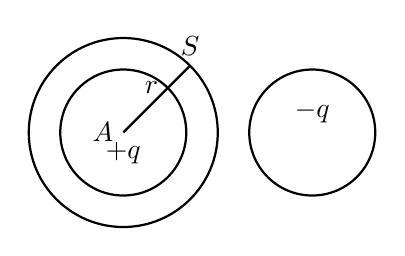
\begin{tikzpicture}
    \draw [thick] (0,0) circle (0.8);
    \draw [thick] (0,0) circle (1.2);
    \draw [thick] (2.4,0) circle (0.8);
    \draw [thick] (0,0)--(0.85,0.85);
    \node [anchor=east] at (0,0) {$A$};
    \node [anchor=north] at (0,0) {$+q$};
    \node [anchor=east] at (0.566,0.566) {$r$};
    \node [anchor=south] at (0.85,0.85) {$S$};
    \node [anchor=south] at (2.4,0) {$-q$};
    \end{tikzpicture}
\end{center}
\end{minipage}
\begin{solution}
    由高斯定理,通过$S$面的电场强度通量为$\frac{q}{\varepsilon_0}$;$S$面上各点的场强由$+q$和$-q$所激发.\sokka{D}
\end{solution}
}
\section{填空题(每空2分,共24分)}
{
\hspace{-2.16em}
\begin{minipage}{0.67\textwidth}
\begin{exercise}{2}{角动量守恒}
一根长为$l$的细绳的一段固定于光滑水平面上的$O$点,另一端系一质量为$m$的小球,开始时绳子是松弛的,小球与$O$点的距离为$h$.使小球以某个初速率沿该光滑水平面上一直线运动,该直线垂直于小球初始位置与$O$的连线.当小球与$O$点的距离达到$l$时,绳子绷紧而使小球沿着另一个以$O$点为圆心的圆形轨道运动,则小球作圆周运动时的动能$E_k$与初动能$E_{k_0}$的比值$\frac{E_k}{E_{k_0}}=$\ans{$\frac{h^2}{l^2}$}.
\end{exercise}
\end{minipage}
\hfill
\begin{minipage}[c]{0.33\textwidth}
\begin{center}
    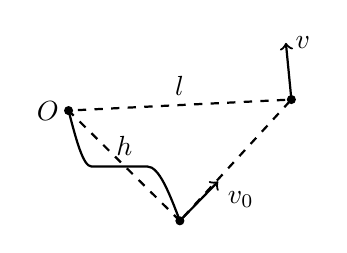
\begin{tikzpicture}
    \filldraw (0,0) circle (0.05);
    \filldraw (2.83,0.14) circle (0.05);
    \filldraw (1.414,-1.4) circle (0.05);
    \draw [thick,dashed] (1.414,-1.4)--(0,0) --(2.83,0.14)--cycle;
    \draw [thick] (0,0) sin (0.29,-0.71) cos (0.71,-0.71) sin (1,-0.71) cos (1.414,-1.4);
    \draw [thick,->] (2.83,0.14) -- (2.76,0.86);
    \draw [thick,->] (1.414,-1.4) -- (1.9,-0.9);
    \node [anchor=north west] at (1.9,-0.9) {$v_0$};
    \node [anchor=west] at (2.76,0.86) {$v$};
    \node [anchor=south] at (1.41,0.07) {$l$};
    \node [anchor=south] at (0.71,-0.7) {$h$};
    \node [anchor=east] at (0,0) {$O$};
    \end{tikzpicture}
\end{center}
\end{minipage}
\begin{solution}
    由于绳子绷紧后拉力始终指向$O$点,故小球对$O$点角动量守恒
    $$mv_0h=mvl$$
    由于动能和速度平方成正比,所以动能之比为
    $$\frac{E_k}{E_{k_0}}=\frac{v^2}{v_0^2}=\frac{h^2}{l^2}$$
\end{solution}

\hspace{-2.16em}
\begin{minipage}{0.67\textwidth}
\begin{exercise}{4}{转动定律,圆周运动}
    如图所示,一质量为$m$、半径为$R$的薄圆盘,可绕通过其一直径的光滑固定轴$AA^{\prime}$转动,转动惯量$I=\frac{mR^2}{4}$.该圆盘从静止开始在恒力矩$M$作用下转动,$t$秒后位于圆盘边缘上与轴$AA^{\prime}$的垂直距离为$R$的$B$点的切向加速度$a_{\tau}=$\ans{$\frac{4M}{mR}$},法向加速度$a_n=$\ans{$\frac{16M^2t^2}{m^2R}$}.
\end{exercise}
\end{minipage}
\hfill
\begin{minipage}[c]{0.33\textwidth}
\begin{center}
    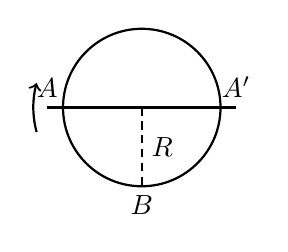
\begin{tikzpicture}
    \draw [thick] (0,0) circle (1);
    \draw [very thick] (-1.2,0)--(1.2,0);
    \draw [thick,densely dashed] (0,0)--(0,-1);
    \node [anchor=south] at (-1.2,0) {$A$};
    \node [anchor=south] at (1.2,0) {$A^{\prime}$};
    \node [anchor=west] at (0,-0.5) {$R$};
    \node [anchor=north] at (-0,-1) {$B$};
    \draw [xshift=-5,thick,<-] (-1.16,0.31) arc (165:195:1.2);
    \end{tikzpicture}
\end{center}
\end{minipage}
\begin{solution}
    由转动定律得圆盘的角加速度$\beta=\frac{M}{I}=\frac{4M}{mR^2}$.则$B$点切向加速度为$a_{\tau}=\beta R=\frac{4M}{mR}$;$t$秒后圆盘的角速度$\omega=\beta t=\frac{4M}{mR^2}t$,$B$点的法向加速度为$a_n=\omega^2R=\frac{16M^2t^2}{m^2R}$.
\end{solution}

\hspace{-2.16em}
\begin{minipage}{0.67\textwidth}
\begin{exercise}{6}{高斯定理,场强计算}
    一均匀带电直导线长为$d$,电荷线密度为$+\lambda$.过导线中点$O$作一半径为$R$($R>\frac{d}{2}$)的球面$S$,$P$为带电直导线的延长线与球面$S$的交点.则通过该球面的电场强度通量$\Phi_e=$\ans{$\frac{\lambda d}{\varepsilon_0}$},带电直线的延长线与球面交点$P$处的电场强度的大小为\ans{$\frac{\lambda d}{4\pi\varepsilon_0\ab(R^2-d^2/4)}$},方向\ans{沿矢径$\boldsymbol{OP}$}.
\end{exercise}
\end{minipage}
\hfill
\begin{minipage}[c]{0.33\textwidth}
\begin{center}
    \begin{tikzpicture}[scale=0.83]
    \draw (0,0) circle (2);
    \draw [thick,->] (-2,0)--(0,0)--(1,1.732);
    \node [anchor=east] at (-2,0) {$P$};
    \filldraw (-2,0) circle (0.05);
    \node [anchor=west] at (0.5,0.866) {$R$};
    \filldraw [pattern=north east lines] (-0.8,-0.1)--(-0.8,0.1)--(0.8,0.1)--(0.8,-0.1)--cycle;
    \draw [thick,|<-] (-0.8,-0.3)--(-0.25,-0.3);
    \draw [thick,|<-] (0.8,-0.3)--(0.25,-0.3);
    \node at (0,-0.3) {$L$};
    \end{tikzpicture}
\end{center}
\end{minipage}
\begin{solution}
    本题第一空考查高斯定理的概念;第二空对带电线$x\sim x+\d x$的一段线元,其电荷量$\d q=\lambda\d x$,与$P$点的距离为$R-x$,在$P$处产生的场强大小为$\d E=\frac{1}{4\pi\varepsilon_0}\frac{\d q}{\left(R-x\right)^2}$,对其积分得
    $$
    \begin{aligned}
        E&=\int_{-d/2}^{d/2} \frac{1}{4\pi\varepsilon_0}\frac{\lambda\d x}{\left(R-x\right)^2}\\
        &=\frac{\lambda d}{4\pi\varepsilon_0\ab(R^2-d^2/4)}
    \end{aligned}
    $$
    方向水平向左(沿矢径$\boldsymbol{OP}$).
\end{solution}

}
\newpage
\section{计算题(共46分)}
{
\hspace{-2.16em}
\begin{minipage}{0.67\textwidth}
    \begin{exercise}{5}{冲量与动量定理}
        如图所示,传送带以$3\mathrm{m/s}$的速率水平向右运动,砂子从高$h=0.8\mathrm{m}$处落到传送带上,即随之一起运动.求传送带给砂子的作用力方向($g=10\mathrm{m/s}^2$).
    \end{exercise}
\end{minipage}
\hfill
\begin{minipage}[c]{0.33\textwidth}
\begin{center}
    \begin{tikzpicture}[scale=0.86]
    \draw [|<->|,thick] (-0.3,0)--(-0.3,2);
    \node [anchor=west] at (-0.3,1) {$h$};
    \draw [thick] (0,0)--(2.5,0) arc (90:-90:0.2) -- (0,-0.4) arc (270:90:0.2)--cycle;
    \draw [->,thick] (0.8,-0.12)--(1.7,-0.12);
    \draw [<-,thick] (0.8,-0.52)--(1.7,-0.52);
    \draw [thick] (0,-0.2) circle (0.2);
    \draw [thick] (2.5,-0.2) circle (0.2);
    \filldraw [pattern=north east lines] (0,0)--(2.5,0)--(2.4,0.1)--(0.1,0.1)--cycle;
    \draw [thick] (-0.2,2.5)--(0,2)--(1.5,2)--(1.7,2.5);
    \end{tikzpicture}
\end{center}
\end{minipage}
\begin{solution}
    质量为$\d m$的砂子在接触传送带前的速度为$v=\sqrt{2gh}$,方向竖直向下.
    $$\vv{p}=-\sqrt{2gh}\d m\boldsymbol{j}=-4\mathrm{m/s}\boldsymbol{j},\ \vv{p}^{\prime}=3\mathrm{m/s}\cdot\d m\boldsymbol{i}$$
    砂子的动量变化为
    $$\Delta\vv{p}=\vv{p}^{\prime}-\vv{p}=3\mathrm{m/s}\d m\boldsymbol{i}+4\mathrm{m/s}\d m\boldsymbol{j}$$
    由动量定理,砂子所受传送带的作用力方向与砂子的冲量变化方向相同(不考虑重力),其夹与水平面的夹角为
    $$\tan{\theta}=\frac{\sqrt{2gh}\d m}{3\mathrm{m/s}\d m}=\frac{\sqrt{2gh}}{3}=\frac{4}{3},\ \theta=\arctan{\frac{4}{3}}=53^{\circ}$$
    方向斜向上.
\end{solution}

\hspace{-2.16em}
\begin{minipage}{0.67\textwidth}
    \begin{exercise}{10}{场强计算}
        真空中两条平行的“无限长”均匀带电直线相距为$a$,其电荷线密度分别为$-\lambda$和$+\lambda$.试求
        \begin{enumerate}
            \item 在两直线构成的平面上,两线间任一点的电场强度(选$Ox$轴如图所示,两线的中点为原点).
            \item 两带电直线上单位长度之间的相互吸引力.
        \end{enumerate}
    \end{exercise}
\end{minipage}
\hfill
\begin{minipage}[c]{0.33\textwidth}
\begin{center}
    \begin{tikzpicture}
    \draw [thick,->] (-2,0)--(2,0);
    \draw [thick] (-1.2,-1.5)--(-1.2,1.5);
    \draw [thick,densely dashed] (-1.2,-2)--(-1.2,-1.5);
    \draw [thick,densely dashed] (-1.2,1.5)--(-1.2,2);
    \draw [thick] (1.2,-1.5)--(1.2,1.5);
    \draw [thick,densely dashed] (1.2,-2)--(1.2,-1.5);
    \draw [thick,densely dashed] (1.2,1.5)--(1.2,2);
    \filldraw [black] (0,0) circle (0.05);
    \node [anchor=north] at (2,0) {$x$};
    \node [anchor=north] at (0,0) {$O$};
    \node [anchor=south] at (-1.2,2) {$-\lambda$};
    \node [anchor=south] at (1.2,2) {$+\lambda$};
    \length{(-1.2,1)}{(1.2,1)}{$a$}
    \end{tikzpicture}
\end{center}
\end{minipage}
\begin{solution}
    \begin{enumerate}
        \item 根据无限长均匀带电直线在线外离直线距离$r$处的场强表达式,$x$处的场强由$-\lambda$和$+\lambda$的带电直线所产生
        $$E=-\frac{\lambda}{2\pi\varepsilon_0\ab(x+a/2)}+\frac{\lambda}{2\pi\varepsilon_0\ab(a/2-x)}=\frac{2a\lambda}{\pi\varepsilon_0\ab(a^2-4x^2)}$$
        \item 单位长度间相互吸引力即一条直线直线在另一条直线所产生电场中的受力大小,即$F=\lambda E=\frac{\lambda^2}{2\pi\varepsilon_0a}$.
    \end{enumerate}
\end{solution}
}